\documentclass[a4paper]{article}

%% Language and font encodings
\usepackage[english]{babel}
\usepackage[utf8x]{inputenc}
\usepackage[T1]{fontenc}

%% Sets page size and margins
%\usepackage[a4paper,top=3cm,bottom=2cm,left=3cm,right=3cm,marginparwidth=1.75cm]{geometry}

%% Useful packages
\usepackage{amsmath}
\usepackage{pgfplots}
\pgfplotsset{compat=1.14}
\usepackage{graphicx}
\usepackage[colorinlistoftodos]{todonotes}
\usepackage[colorlinks=true, allcolors=blue]{hyperref}
\usepackage{subfig}
\usepackage{float}
\usepackage{multicol}


\title{\vspace{-3em}COMS30121 - Image Processing and Computer Vision\\The Dartboard Challenge\vspace{-0.3em}}
\author{Joshua Van Leeuwen \& Karim Allaouat}
\date{}

\usepackage{titlesec}
\usepackage[margin=0.5in]{geometry}
\geometry{top=10mm, bottom=17mm}

\begin{document}
\vspace{-10em}
\maketitle
\vspace{-4em}

\setcounter{section}{-1}
\section*{Introduction}

This task introduces the ability to detect and locate instances of an object
class in images. This is important as this ability is used in many computer
vision applications. The task explores the Viola-Jones object detection
framework (an “off the shelf” face detector) and combines it with other
detection techniques to improve it. The image set used is from the popular
sport, darts.

\section*{The Viola-Jones Object Detector}

The Viola-Jones object detection framework is the first object detection
framework to provide competitive object detection rates in real time. The
algorithm was used with a strong classifier trained using AdaBoost for
detecting human faces from the front.

\subsection*{Using the Detector on Human Faces}
\vspace{-0.7em}

\begin{figure}[H]
  \centering
  \subfloat[dart4.jpg.]{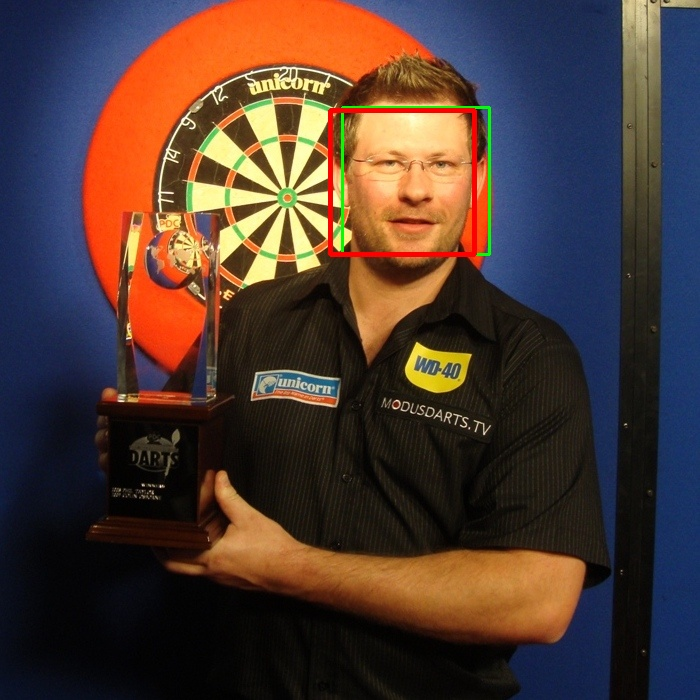
\includegraphics[width=\textwidth, height=20mm, keepaspectratio]{task1/out4.jpg}\label{fig:dart4}}
  \hfill
  \subfloat[dart5.jpg]{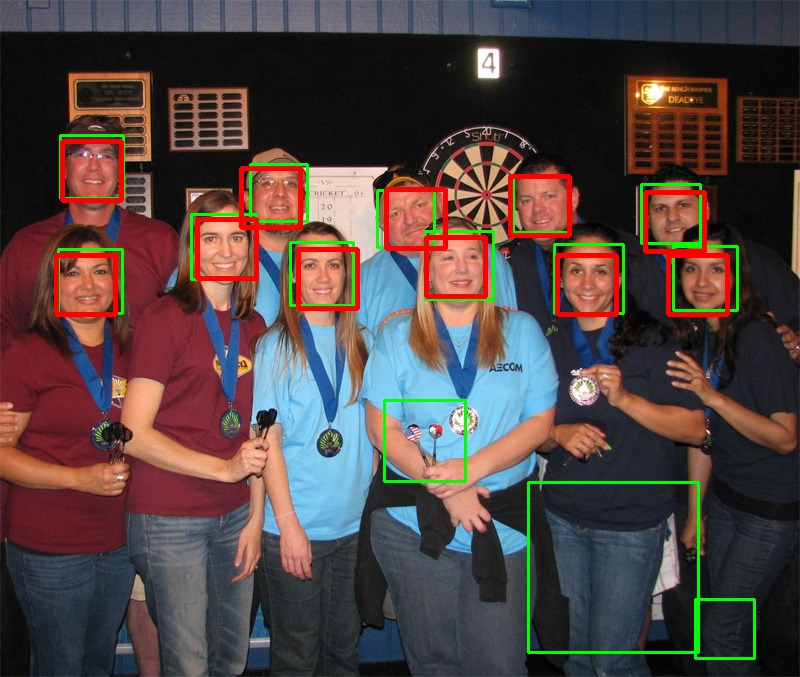
\includegraphics[width=\textwidth, height=20mm, keepaspectratio]{task1/out5.jpg}\label{fig:dart5}}
   \hfill
  \subfloat[dart13.jpg]{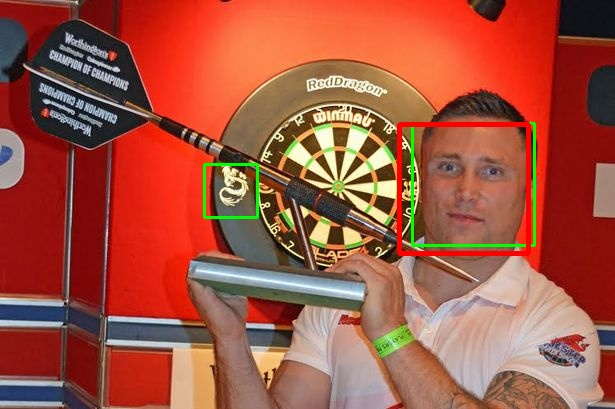
\includegraphics[width=\textwidth, height=20mm, keepaspectratio]{task1/out13.jpg}\label{fig:dart13}}
   \hfill
  \subfloat[dart14.jpg]{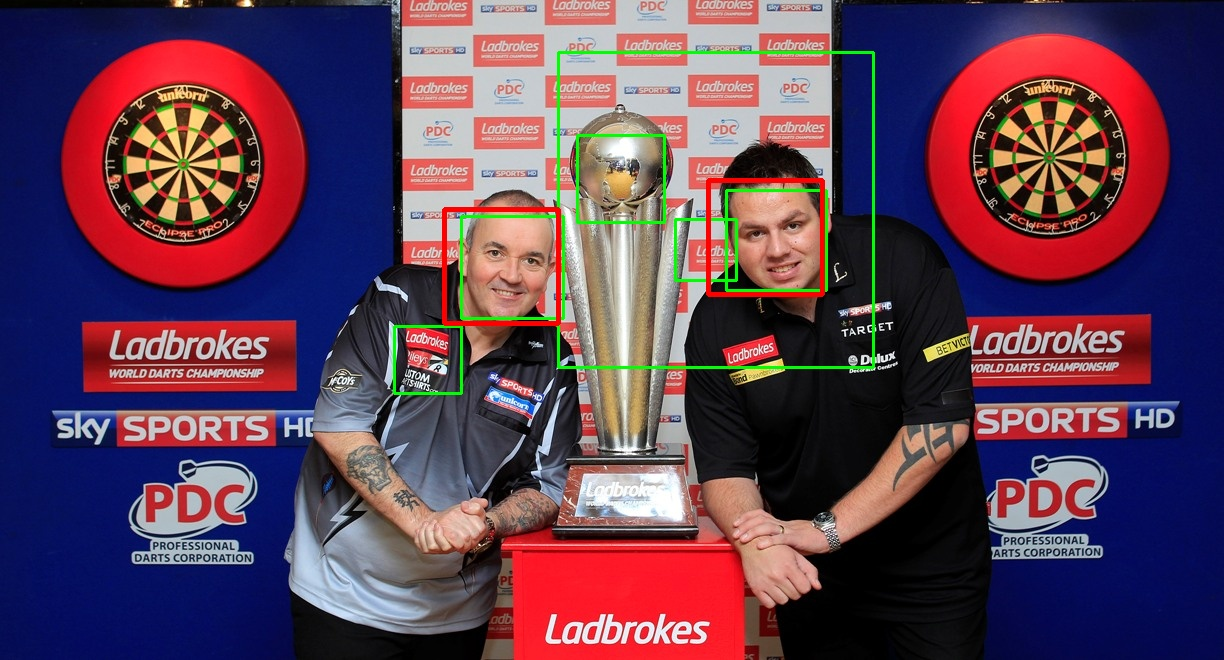
\includegraphics[width=\textwidth, height=20mm, keepaspectratio]{task1/out14.jpg}\label{fig:dart14}}
   \hfill
  \subfloat[dart15.jpg]{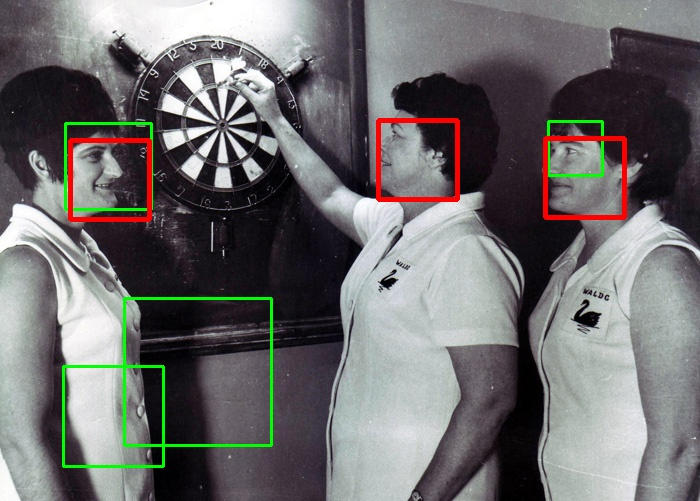
\includegraphics[width=\textwidth, height=20mm, keepaspectratio]{task1/out15.jpg}\label{fig:dart15}}
   \hfill
   \caption{Result of the Viola-Jones Algorithm on human faces (green boxes). Red boxes represent ground truth.}
\end{figure}

\subsection*{Assessing How the Detector Performs}
\vspace{-0.7em}

The TPR or True Positive Rate measures the proportion of relevant items that
are correctly identified. In this case it is the fraction of successfully
detected faces out of all valid faces in an image. The TPR of dart5.jpg and
dart15.jpg are 100\% and 67\% respectfully.

A practical difficulty of computing the TPR accurately is that the hits and
misses have to be manually counted. Also, errors can occur when faces are side
profile because they become ambiguous as to whether they are valid. It is
always possible to get 100\% TRP because you can detect everything in the image
and so will always get all possible hits. It will however, get all the misses
too. A better way of evaluating the detector would be to calculate the
\(F_{1}\) score. It takes into account the detectors precision (PPV - Positive
Prediction Value, how many selected items are relevant) and recall (TPR). A set
of rules were created to evaluate whether a face was valid:


\begin{itemize}
  \item Two eyes and a mouth must be within a boundary to be counted as a hit.
  \item Two eyes and a mouth must be visible to us in order for it to be
    counted as valid.
  \item The \(F_{1}\) score will be calculated by: \[\frac{2 \times P \times
    R}{R + P}\] Where
  \item Recall (TPR) ${P = \frac{true positives}{ground truth}}$.
  \item Precision ${R = \frac{true positives}{true positives + false
    positives}}$.
\end{itemize}

As calculating the F1 score is challenging due to manually counting boxes, a process was implemented that makes this easier and scalable. It will compare the centres of the ground truth (which are manually added) and detection boxes and if they are below a certain threshold, will count as a true positive. Table 1 below shows the result of this.

\begin{table} [H]
\centering
\begin{tabular}{l| r | r | r | r | r | r}
Picture & Actual & Detected & Hit & Missed & \(F_{1}\) Score \\\hline
dart4 & 1 & 1 & 1 & 0 & 1\\
dart5 & 11 & 14 & 11 & 3 & 0.88 \\
dart13 & 1 & 2 & 1 & 1 & 0.67 \\
dart14 & 2 & 6 & 2 & 4 & 0.5 \\
dart15 & 3 & 4 & 2 & 2 & 0.5
\end{tabular}
\caption{\label{tab:F1}Comparing the \(F_{1}\) Score of different images.}
\end{table}

\section*{Building and Testing the Detector}
\subsection*{Interpreting TPR vs FPR}
\vspace{-0.7em}

Figure 2 shows the training of the detector over the 3 stages. The TPR always
remained as 1 therefore, it was successful in detecting all dartboards. The
decreasing FPR portrays that the detector firstly detects as much as it can,
then reduces the number of objects it detects. As a consequence, it is clear
that the detector is improving. The parameters of the detector were changed to be optimum. A ratio of 500:1000, positive to negative was used and a max false alarm rate of 0.4. TODO: explain parameter tuning.

\begin{figure}[H]
  \centering
  \begin{tikzpicture}
    \begin{axis}[
      title=TPR vs FPR,
      xlabel=$Stage$,
      ylabel=$Rate$
    ]
      \addplot table {task2/TPR.dat};
      \addplot table {task2/FPR.dat};
    \end{axis}
  \end{tikzpicture}
  \caption{TPR (blue) vs FPR (red) across the 3 stages.}
\end{figure}

\subsection*{Testing on images}
\vspace{-0.7em}

\begin{figure}[H]
  \centering
  \subfloat[dart4.jpg.]{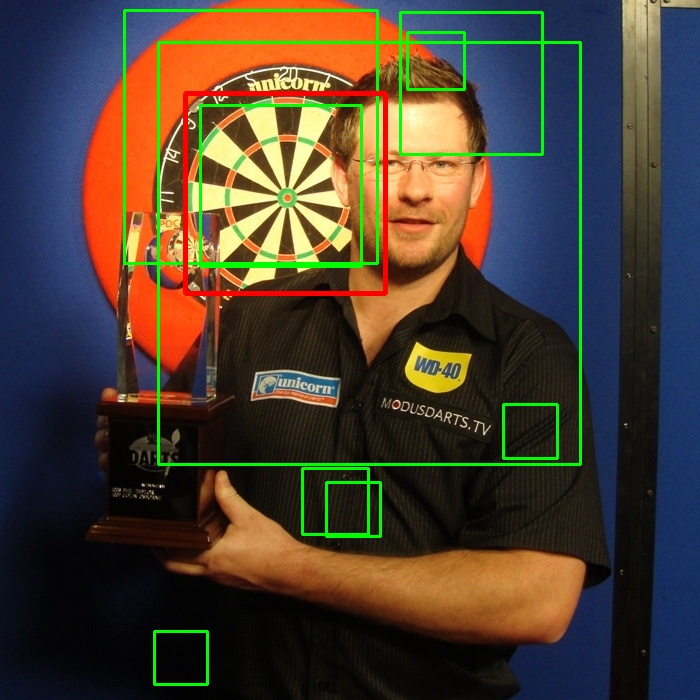
\includegraphics[width=\textwidth, height=20mm, keepaspectratio]{task2/out4.jpg}\label{fig:out4}}
  \hfill
  \subfloat[dart5.jpg]{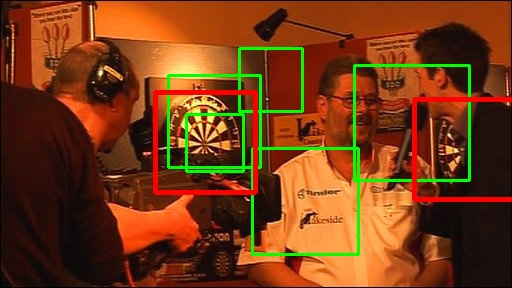
\includegraphics[width=\textwidth, height=20mm, keepaspectratio]{task2/out11.jpg}\label{fig:out11}}
   \hfill
  \subfloat[dart13.jpg]{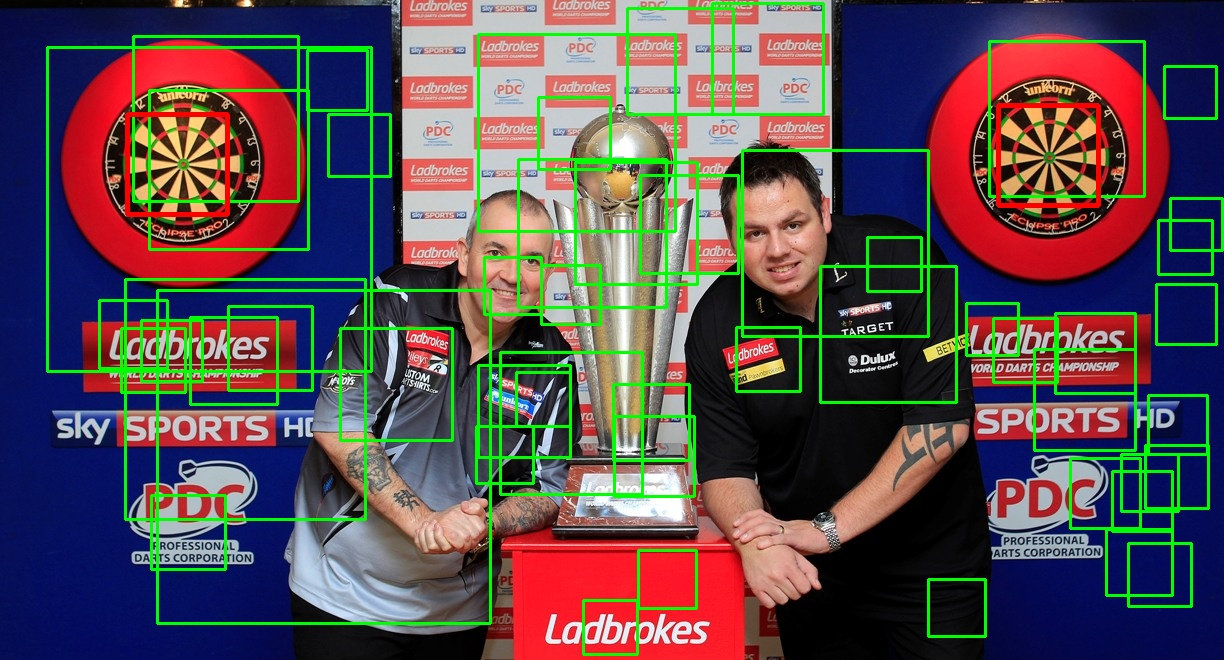
\includegraphics[width=\textwidth, height=20mm, keepaspectratio]{task2/out14.jpg}\label{fig:out14}}
   \hfill
  \subfloat[dart14.jpg]{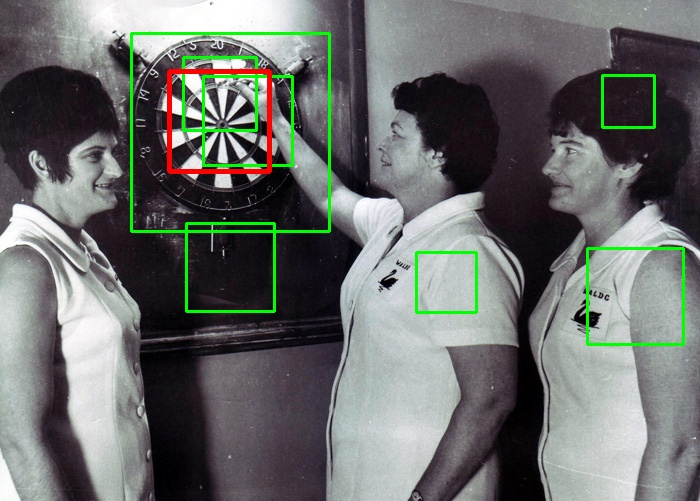
\includegraphics[width=\textwidth, height=20mm, keepaspectratio]{task2/out15.jpg}\label{fig:out15}}
   \hfill
   \caption{Result of the trained dartboard detector.}
\end{figure}

TODO: make this look beter?\newline
The \(F_{1}\) of the images are:
\begin{multicols}{4}
    \begin{itemize}
		\item dart0.jpg - 0.14.
        \item dart1.jpg - 0.13.
        \item dart2.jpg - 0.12.
        \item dart3.jpg - 0.20.
        \item dart4.jpg - 0.20.
        \item dart5.jpg - 0.10.
        \item dart6.jpg - 0.17.
        \item dart7.jpg - 0.09.
        \item dart8.jpg - 0.13.
        \item dart9.jpg - 0.13.
        \item dart10.jpg - 0.11.
        \item dart11.jpg - 0.29.
        \item dart12.jpg - 0.33.
        \item dart13.jpg - 0.14.
        \item dart14.jpg - 0.07.
        \item dart15.jpg - 0.25.
    \end{itemize}
\end{multicols}

The overall \(F_{1}\) score is consequently 0.1625. The \(F_{1}\) score is relatively low therefore the denominator is much bigger
and can conclude that there was a high number of detections with respect to hits. This means that there were a lot of misses. The usefulness of the plot (Figure 2) is that it can be clearly seen that the detector is currently under fitting as the TPR remains at 1 and the FPR decreases. This fact, along with the \(F_{1}\) scores, portray the results of a poor detector. However, it can be used to an advantage. The under fitting can be combined with other classifying detectors in order to improve results.

\section*{Integration with Shape Detectors}
\subsection*{Image Results}
\vspace{-0.7em}

\begin{figure}[H]
  \centering
  \subfloat[Threshold Gradient Magnitude.]{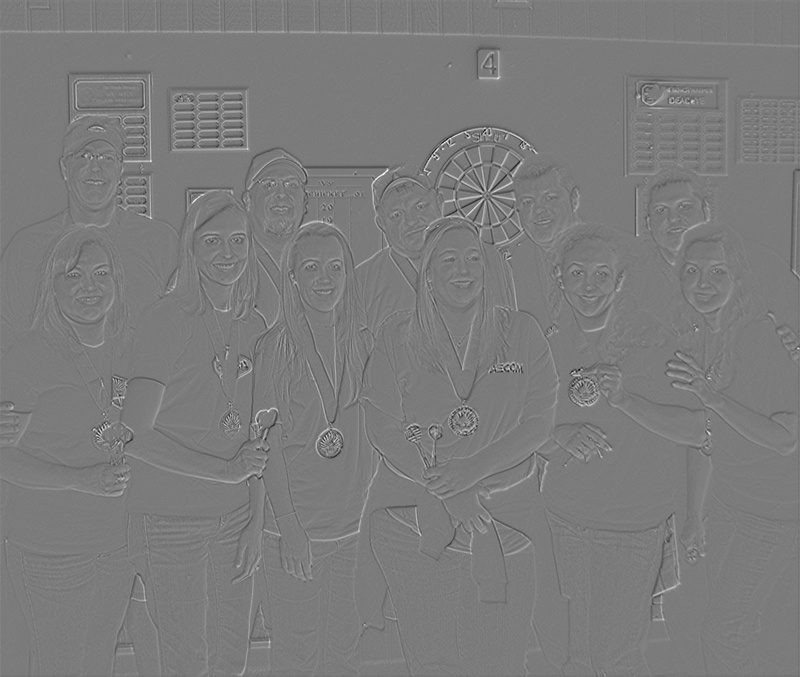
\includegraphics[width=\textwidth, height=20mm, keepaspectratio]{task3/mag5.jpg}\label{fig:mag1}}
  \hfill
  \subfloat[Hough Space]{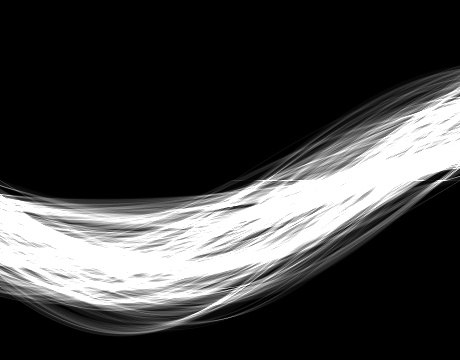
\includegraphics[width=\textwidth, height=20mm, keepaspectratio]{task3/hough5.jpg}\label{fig:hough1}}
   \hfill
  \subfloat[Result]{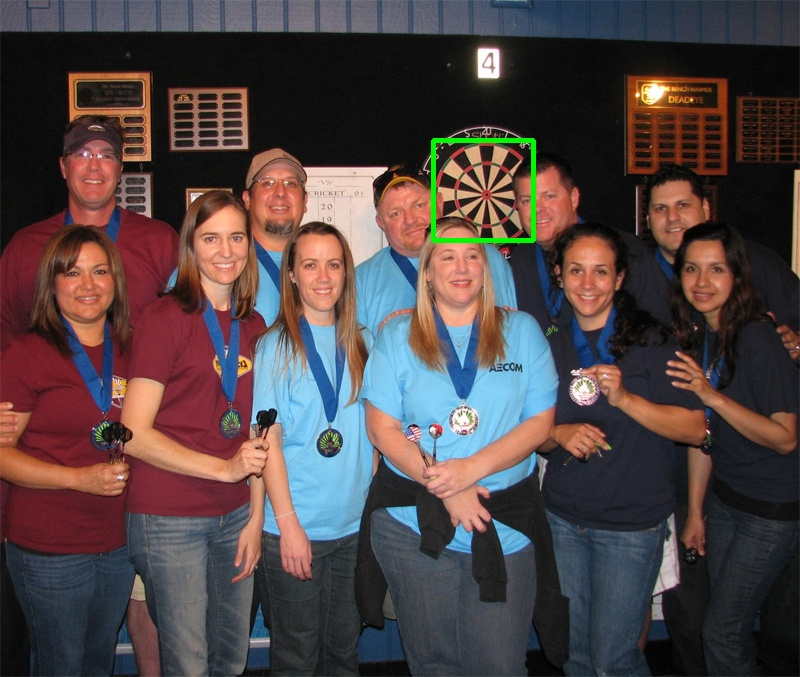
\includegraphics[width=\textwidth, height=20mm, keepaspectratio]{task3/out5.jpg}\label{fig:result1}}
   \hfill
   \caption{dart5.jpg shows the merits of the detector.}
\end{figure}

\begin{figure}[H]
  \centering
  \subfloat[Threshold Gradient Magnitude.]{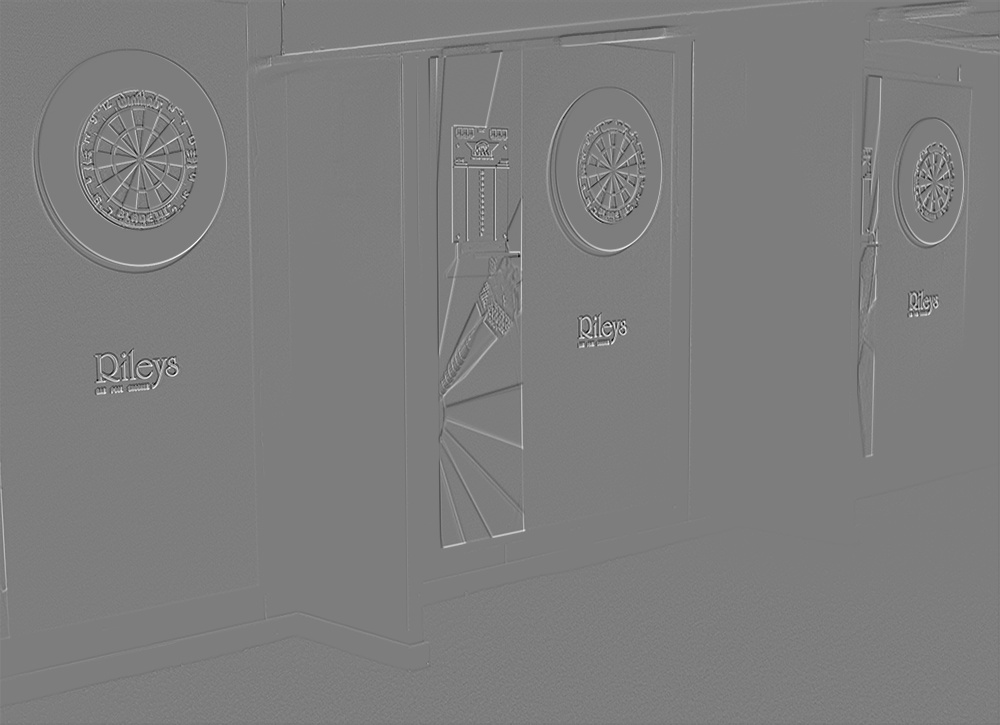
\includegraphics[width=\textwidth, height=20mm, keepaspectratio]{task3/mag10.jpg}\label{fig:mag2}}
  \hfill
  \subfloat[Hough Space]{
\includegraphics[width=\textwidth, height=20mm, keepaspectratio]{task3/hough10.jpg}\label{fig:hough2}}
   \hfill
  \subfloat[Result]{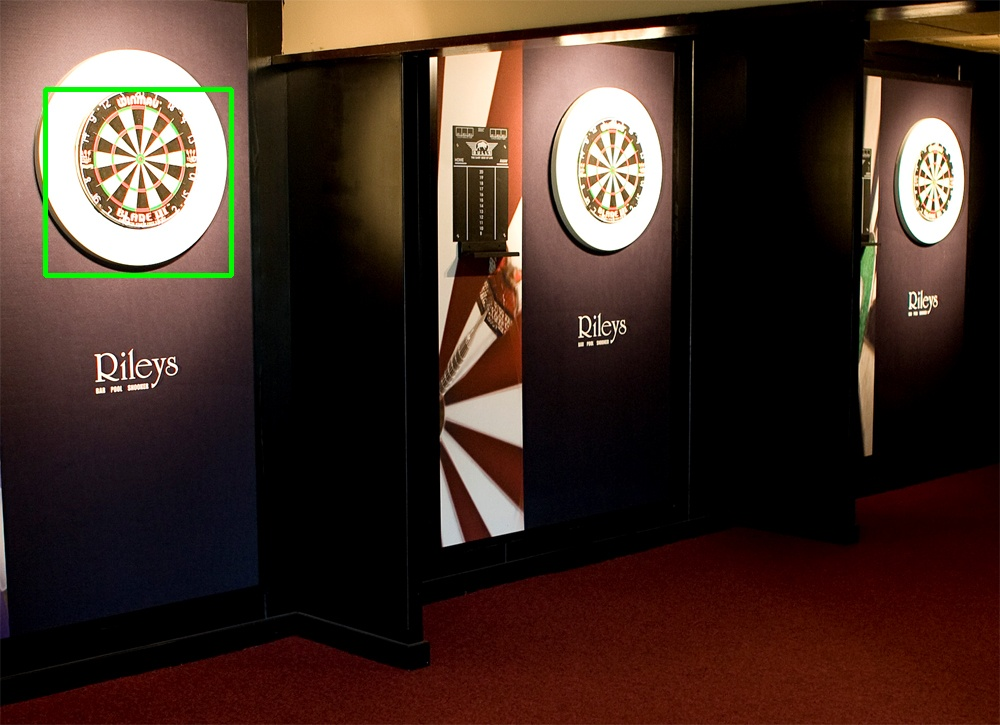
\includegraphics[width=\textwidth, height=20mm, keepaspectratio]{task3/out10.jpg}\label{fig:result2}}
   \hfill
   \caption{dart10.jpg shows the limitations of the detector.}
\end{figure}


\subsection*{Merits and Limitations}
\vspace{-0.7em}
The new dartboard detector did considerably better than the previous, achieving
an overall \(F_{1}\) score 0.767 with the previous being 0.1625. This detector adds more classifiers when analysing images meaning that
the large set of detections with many negative hits, is able to be reduced by
combining each classifier result. This detector works optimally with images
where dartboards are in good lighting and are facing straight at the camera in
the scene. As shown in the dart10.jpg image, the detector failed to detect two
dartboards that are at an angle. This is because of the circle and line Hough
transformation being used, struggle to detect these. TODO: Talk about how we get the line detections - intersections etc.

\subsection*{Combination of Detectors}
\begin{figure}[H]
  \centering
  \subfloat[Flowchart representing the detector.]{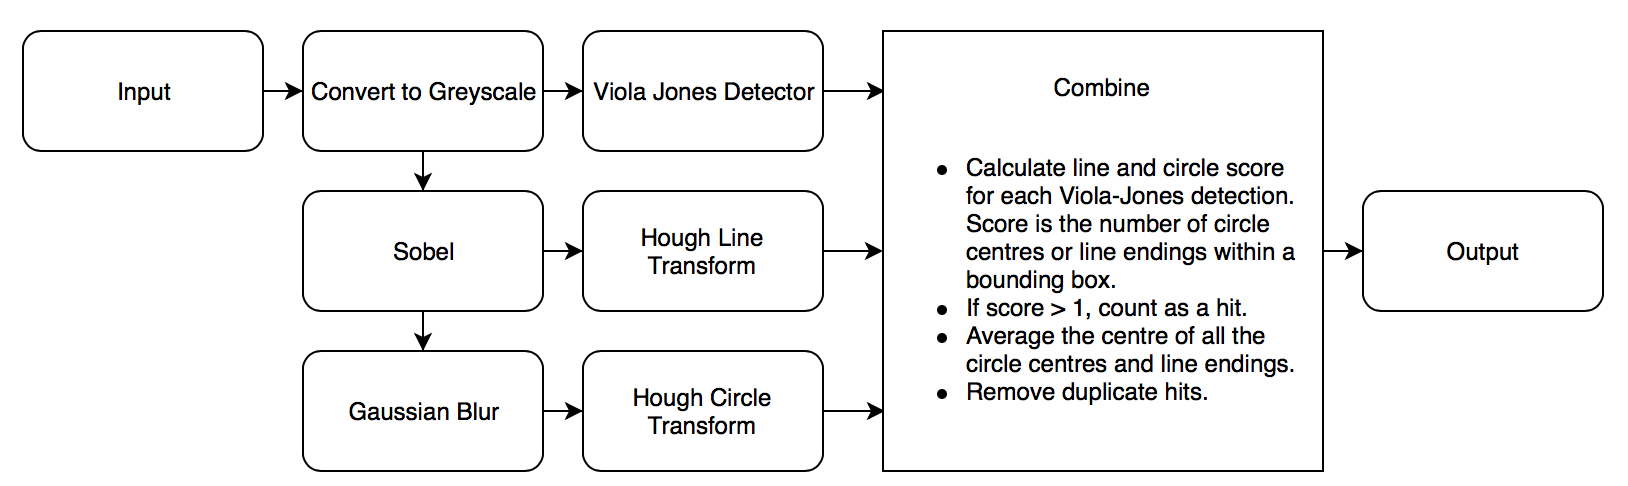
\includegraphics[width=\textwidth, height=40mm, keepaspectratio]{task3/flowchart.png}\label{fig:flowchart}}
\end{figure}

As shown, the Viola Jones detector results have a positive detection of every
dartboard in each image however, have a large amount of false positives. The 
approach was to create new classifiers which would refine these hits down to
true positives by accepting Viola Jones hits that were also observed by the
line and circle detectors. This involves iterating through the set of Viola
hits, comparing whether any line or circle hits are contained in the Viola
bounding box, accepting if so, rejecting otherwise. If accepted, this hit would
change its location based on the average position of itself, along with its
combined detections. With the use of the circle detections, it also has the ability to estimate the size of the dartboard. Furthermore, it takes the average
radii of included circles and includes this in the approximation.  Once the new set of accepted detections had been achieved, it was clear that multiple
bounding boxes overlapped with one another. Therefore, all bounding boxes
that were overlapping were combined, again averaging the coordinates and size - ensuring one
positive hit per dartboard.



\section*{Improving the Detector}

\begin{itemize}
\item In order to improve our dartboard classifier, we considered further shapes
which help to classify a dartboard being present.  As such, we identified two
shapes - ellipses and triangles. Firstly, we realised that some dartboards
had been not been identified by our classifier due to not being detected by
circles with dartboards that are at an angle.  By using ellipses, we would
be able to capture this shape of valid dartboards. We also chose to consider
triangle shapes inside images to detect dartboards.  This is because all
dartboards have distinct triangles contained that will give more detections
that can be combined in our detector.

\item Detecting both triangle and ellipse shapes is achieved by first applying the
Canny edge detector on the grey scale input image.  The Canny edge detector,
developed by  John F. Canny in 1986 [1] and works by calculating
the gradient magnitude of each pixel. To determine whether each pixel is part
of an edge, two thresholds are applied where; pixels greater than the high threshold
are considered pixels on an edge, pixels below the low threshold are
discarded and pixels in-between the two thresholds are considered edges only if
they are connected to a pixel that is above the higher threshold. In order to
select an appropriate threshold for each image, the Otsu method can be applied.
[2]

\item The Otsu method is used to determine the largest threshold input for the Canny
edge detector and it assumes that the image contains two classes of pixels. It then calculates the optimum threshold and partitions the two classes so that their combined 
variance is maximal. Canny recommended a upper:lower ratio between 2:1 and 3:1 so we decided that the lower threshold value is one third of the returning value from the Otsu method. 

\item TODO: Surf Method. We use a scoring system with surf. We cluster surfs together that count as the same object.

\item TODO: find better viola jones parameters.

\item Include images to show off improvements.

\item After implementing this the F1 score became 0.86666673333333333333.

\end{itemize}

\section*{References}

\begin{enumerate}
\item http://citeseerx.ist.psu.edu/viewdoc/download?doi=10.1.1.420.3300\&rep=rep1\&type=pdf
\item https://en.wikipedia.org/wiki/Otsu\%27s\_method
\end{enumerate}

\vspace{-4em}
\end{document}
